\begin{definition}[Polinomios con coeficientes en un anillo conmutativo]
Dado un anillo commutativo A y un símbolo X no usado para representar elementos de A. 

Un polinomio es una función de coeficientes $f: \mathbb{N} \to A$ de soporte finito: $$\exists n \in \mathbb{N}. \forall m > n. f(m) = 0$$ es decir, toma valor no nulo en un subconjunto finito de $\mathbb{N}$. 

En el conjunto de todos los polinomios sobre $A$ definimos dos operaciones:

\begin{itemize}
\item Suma de polinomios: $(f,g) \mapsto f+g$ tal que $\forall n \in \mathbb{N}.(f+g)(n) = f(n) +g(n)$
\item Producto de polinomios: $(f,g) \mapsto f \cdot g$ tal que $ \forall n \in \mathbb{N}.(f \cdot g)(n) = \sum_{i+j = n} f(i) g(j)$
\end{itemize}
\end{definition}

\begin{proposition}[Estructura de anillo conmutativo de los polinomios]
El conjunto $A[X]$ de los polinomios con coeficientes en $A$ es un anillo conmutativo. 
\end{proposition}
\begin{proof}
Claramente, las operaciones son internas:

Dados $f,g \in A[X]$ tenemos que $\exists. n_f,n_g$ tales que $\forall n > n_f. f(n) = 0 \land \forall n > n_g. g(n) = 0$. 

Tomando $n_+ = max\{n_f,n_g\}$ tenemos que $\forall n > n_+. (f+g)(n) = f(n)+g(n) = 0$. Por tanto, $f+g \in A[X]$. 
Tomando $n_\cdot = n_f + n_g$ tenemos que $\forall n > n_\cdot. (f \cdot g)(n) = \sum_{i+j = n} f(i)g(j)$ dado que $i,j \in \mathbb{N} \land i+j > n_f + n_g$ necesariamente $i > n_f \lor j > n_g$ en cuyo caso todos los términos $f(i)g(j)$ son cero. Por tanto, $f \cdot g \in A[X]$. 

Las propiedades de asociatividad para la suma y la commutividad son fáciles de ver. Veamos como se demuestra la asociatividad para el producto:

$(f(gh))(n) = \sum_{i+m = n} f(i)(gh)(m) = \sum_{i+m = n} f(i) (\sum_{j+k = m} g(j)h(k)) = \sum_{i+m = n \land j+k = m} f(i)g(j)h(k) = \sum_{i+j+k = m} f(i)g(j)h(k)$. Donde la última igualdad se verifica por la propiedad de distributividad generalizada. 

El elemento neutro para la suma es el polinomio $0: \mathbb{N} \to A$ tal que $\forall n \in \mathbb{N}. 0(n) = 0$. 

El elemento neutro para el producto es el polinomio $1:\mathbb{N} \to A$ tal que $1(0) = 1 \land \forall n > 0. 1(n) = 0$. En efecto, $(f\cdot 1)(n) = \sum_{i+j = n} f(i)1(j) = f(n)1(0) = f(n)$. 

El elemento opuesto de un polinomio $f$ es el polinomio $-f: \mathbb{N} \to A$ tal que $\forall n. (-f)(n) = -f(n)$. 

Se verifica la distributividad de la suma respecto del producto:

$f \cdot (g+h)(n) = \sum_{i+j = n} f(i) (g+h)(j) = \sum_{i+j = n} (f(i)g(j) + f(i)h(j)) = \sum_{i+j = n} f(i)g(j) + \sum_{i+j = n} f(i)h(j) = (f\cdot g + f \cdot h)(n)$.  
\end{proof}

\begin{definition}[Polinomios destacados y grado de un polinomio]
Consideremos un anillo de polinomios $A[X]$. 

Un polinomio $f \in A[X]$ es constante si $\forall n > 0. f(n) = 0$. Si $f(0) = a$ lo denotamos por $a$. 

La potencia k-ésima de x es el polinomio$f: \mathbb{N} \to A$ tal que $f(k) = 1 \land \forall n \neq k. f(n) = 0$. Lo denotaremos por $x^k$. 

Dado $f \neq 0$ un polinomio no nulo. El grado de f es un número natural $n$ tal que $p(n) \neq 0 \land \forall m > n. f(m) = 0$. Por convención al polinomio nulo se le asigna grado $-\infty$.  Al grado de un polinomio $f$ se le denota por $gr(f)$. 

Un polinomio con un único coeficiente no nulo se llama monomio. 
\end{definition}

\begin{proposition}
Si identificamos $A$ con el conjunto de los polinomios constantes, entonces $A$ es un subanillo de $A[X]$. 
\end{proposition}
\begin{proof}
En efecto, las operaciones suma y producto de $A[X]$ son cerradas para el conjunto de los polinomios constantes. También $1,-1$ son polinomios constantes. 
\end{proof}

\begin{lemma}
$\forall k \ge 0, a \in A - \{0\}$, $a \cdot x^k$ es el monomio de grado k con coeficiente a en grado k. 
\end{lemma}
\begin{proof}
La demostración se hace por inducción sobre k. Para $k = 0$, se verifica que $ax^0 = a$. 

Suponiendo que es cierto para $k$ se compruebra que es cierto para $ax^{k+1}$. En efecto, $(ax^{k+1})(n) = ((ax^k)x)(n) = \sum_{i+j = n} (ax^k)(i)x(j) = (ax^k)(n-1)$ y por hipótesis de inducción sabemos que este polinomio vale $a$ si $k = n-1$ y cero en otro caso, luego el polinomio original vale $a$ en k+1 y cero en otro caso. 
\end{proof}

\begin{definition}[Notación de un polinomio como suma de monomios]
Dado $f \in A[X]$ tal qque $\forall n \in \mathbb{N}. f(n) = a_n$. Representamos este polinomio mediante la expresión $\sum_{n \ge 0} a_nx^n$. 
\end{definition}

Podemos comprobar que ambas expresiones representan el mismo polinomio: $$\sum_{n \ge 0} a_n x^m)(m) = \sum_{n \ge 0} (a_n x^n)(m) = (a_mx^m)(m) = a_m = f(n)$$

Usando esta notación multiplicaríamos del siguiente modo: $$(\sum_{n \ge 0} a_n x^n)(\sum_{n \ge 0} b_n x^n) = \sum_{n,m \ge 0} a_n b_m x^{n+m} = \sum_{n \ge 0} (\sum_{n+m = k} a_nb_m) x^k$$ 

\begin{example}
Consideramos $f = 2+5x+4x^2, g = 1+3x \in \mathbb{Z}_6[X]$, claramente $f+g=3+2x+4x^2, -g = 5+3x,f\cdot g = 2 + 5x + x^2$. Nótese que aquí $gr(f \cdot g) \neq gr(f) + gr(g)$. Esta fórmula sólo será cierta cuando el anillo original sea un dominio de integridad. 
\end{example}

\begin{theorem}[Propiedad universal de los anillos de polinomios]
Dados $A,B$ dos anillos conmutativos y un homomorfismo $f: A \to B$. Dado $u \in B$ existe un único homomorfismo de anillos $f_u: A[X] \to B$ tal que $\forall a \in A:f_u(\lambda(a)) = f(a)$ y $f_u(x) = u$. Donde $\lambda$ es la inclusión de $A$ en $A[X]$. 

\begin{figure}[H]
\centering
\makebox[\textwidth][c]{
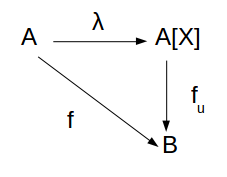
\includegraphics[scale=0.5]{./images/universal.png}
}
\end{figure}
\end{theorem}
\begin{proof}
Dado $p = \sum_{n \ge 0} a_n x^n \in A[X]$, defino $f_u(p) = \sum_{n \ge 0} f(a_n)u^n$, que llamaremos homomorfismo de evaluación. 

Claramente, $f_u$ satisface las propiedades requeridas y su codominio es $B$. Además es un homomorfismo. En efecto, $f_u(1) = 1$ y $$f_u(pq) = f(\sum{n \ge 0} (\sum_{i+j = n a_ib_j} a_ib_j)u^n = \sum_{n \ge 0} f(\sum_{i+j = n} a_ib_j)u^n = \sum_{n \ge 0} (\sum_{i+j = n} f(a_i)f(b_j))u^n$$ donde se ha utilizado la definición de $f_u$ y que $f$ es un homomorfismo y por otro lado $$f_u(p)f_u(q) = (\sum_{n \ge 0} f(a_n) u^n)(\sum_{n \ge 0} f(n_n) u^n) = \sum{i,j \ge 0} f(a_i)u^if(b_j)u^j = \sum_{i,j \ge 0} f(a_i)f(b_j)u^{i+j} = \sum_{n \ge 0} (\sum_{i+j = n} f(a_i)f(b_j))u^n$$ donde se ha utilizado la asociatividad generalizada y el hecho de que el anillo es conmutativo. Claramente, ambas expresiones son iguales. También es fácil demostrar que $f_u(p+q) = f_u(p) + f_u(q)$. 

Finalmente, $f_u$ es el único homomorfismo que verifica las propiedades requiridas. En efecto, si $\phi:A[X] \to B$ verifica $\forall a \in A. \phi(\lambda(a)) = f(a) \land \phi(x) = u$ entonces $$\phi(\sum_{n \ge 0} a_n x^n) = \sum_{n \ge 0} \phi(a_n x^n) = \sum_{n \ge 0} \phi(a_n) \phi(x)^n = \sum_{n \ge 0} f(a_n) u^n = f_u(\sum_{n \ge 0} a_n x^n)$$
\end{proof}

Un caso particular se cuando $A$ es un subanillo de $A$, en este caso $f$ es la inclusión y $f_u$ se denota por $E_u$ y se llama morfismo de evaluación en u. Claramente, $E_u(\sum_{n \ge 0} a_n x^n) = \sum_{n \ge 0} a_n u^n$. Para cualquier polinomio, este homomorfismo permite el cálculo del valor del polinomio en cualquier punto. 

\begin{definition}
Dado un anillo conmutativo $A$ e $Y$ un símbolo que no denota a ningún elemento de $A[X]$. Definimos el anillo de polinomios en dos indeterminadas como $A[X,Y] = A[X][Y] = A[Y][X]$ donde el producto se realiza como $$(\sum_{i,j \ge 0} a_{ij}x^iy^j)(\sum_{k,l \ge 0} b_{kl}x^ky^l) = \sum_{i,j,k,l \ge 0} a_{ij}b_{kl} x^{i+k}y^{j+l} = \sum_{m,n \ge 0} (\sum_{i+k = m \land j+l = n} a_{ij}b_{kl}) x^m y^n$$ donde hemos utilizado la propiedad distributiva generalizada y la propiedad commutativa del producto. 
\end{definition}

\begin{proposition}
La anterior, es una buena definición.
\end{proposition}
\begin{proof}
Dado $f \in A[X][Y]$, $f$ es de la forma $\sum_{j \ge 0} f_j(x) y^j$ con $f_j(x) \in A[X]$, si escribimos $f_j(x) = \sum_{i \ge 0} a_{ij} x^i$ nos queda para $f$: $$f = \sum_{j \ge 0} (\sum_{i \ge 0} a_{ij} x^i) \cdot y^j = \sum_{i,j \ge 0} a_{ij} x^i y^j = \sum_{i,j \ge 0} a_{ij} y^j x^i = \sum_{i \ge 0} (\sum_{j \ge 0} a_{ij} y^j)x^i = \sum_{i \ge 0} g_j(y) x^i \in A[Y][X]$$ donde hemos utilizado la propiedad distributiva generalizada con uno de los factores de longitud uno repetidas veces. Esto demuestra que $A[X][Y] = A[Y][X]$ de donde la definición anterior es buena. 
\end{proof}

\begin{definition}
Definimos inductivamente $A[X_1,\cdots,X_r]$:

Para $r = 1$ no hay nada que definir. Supuesto definido para $r$, $A[X_1, \cdots, X_{r+1}] = A[X_1, \cdots, X_r][X_{r+1}]$.

Los elementos de $A[X_1,\cdots,X_r]$ se expresan como $\sum_{i_1,\cdots,i_r} a_{i_1}\cdots a_{i_r} x_1^{i_1} \cdots x_r^{i_r}$.
\end{definition}

\begin{theorem}[Propiedad universal de los anillos de polinomios multivariados]
Dados $A,B$ dos anillos conmutativos y un homomorfismo $f: A \to B$. Dado $u \in B^k$ existe un único homomorfismo de anillos $f_u: A[X_1,\cdots,X_r] \to B$ tal que $\forall a \in A:f_u(\lambda(a)) = f(a)$ y $f_u(x_i) = u_i$. Donde $\lambda$ es la inclusión de $A$ en $A[X_1,\cdots,X_r]$. 

\begin{figure}[H]
\centering
\makebox[\textwidth][c]{
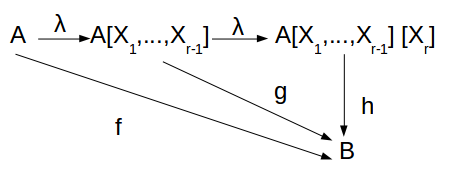
\includegraphics[scale=0.5]{./images/multiuniversal.png}
}
\end{figure}
\end{theorem}
\begin{proof}
Procedemos por inducción sobre $n$. El caso $n = 1$ está demostrado. Supongamos que la propiedad es cierta para $r-1$ y veámoslo para $r$. Dado $u \in B^k$ por hipótesis de inducción existe un único homomorfismo de anillos $g:A[A_1,\cdots,X_{r-1}] \to B$ tal que $\forall a \in A. g(\lambda(a)) = f(a) \land g(x_i) = b_i$ con $1 \le i \le r-1$. Luego aplicamos el caso $n = 1$ con $A = A[X_1,\cdots,X_{r-1}]$ y obtenemos un único homomorfismo $h:A[X_1,\cdots,X_{r-1}][X_r] \to B$ tal que $\forall p \in A[A_1, \cdots,X_{r-1}]. h(\lambda(p)) = g(p) \land g(x_r) = b_r$. Por las características de $g$ está claro que $h$ es un homomorfismo con las propiedades requeridas por el teorema. 
\end{proof}